\documentclass{article}
\usepackage{graphicx}
\usepackage{amsmath}
\usepackage{booktabs}
\usepackage{siunitx}
\usepackage{float}

\title{Assignment 3 - EE4725 Quasi Optical Systems}
\author{Daniel Tyukov \\ Student Number: 5714699 \\ Microelectronics, TU Delft}
\date{March 2026}

\begin{document}

\maketitle

\tableofcontents
\newpage

%% ====================================================================
\section{System Parameters}
%% ====================================================================

The system under analysis is an elliptical dielectric lens antenna with the following parameters:
\begin{itemize}
\item Operating frequency: $f = \SI{200}{GHz}$, wavelength $\lambda_0 = c/f = \SI{1.5}{mm}$, wavenumber $k_0 = 2\pi/\lambda_0$
\item Dielectric material: fused silica, $\varepsilon_r = 4$, wavenumber in dielectric $k_d = \sqrt{\varepsilon_r}\,k_0 = 2k_0$
\item Feed: planar antenna at the lower focal point of an elliptical lens, with Gaussian far field in infinite dielectric:
\begin{equation}\label{eq:feed}
\vec{E}^{a}_{far}(\theta,\phi) = e^{-\left[\left(\frac{u}{u_0}\right)^2 + \left(\frac{v}{v_0}\right)^2\right]} \left(\sin\phi\,\hat{\theta} + \cos\phi\,\hat{\phi}\right) \frac{e^{-jk_d r}}{r}
\end{equation}
where $u = \sin\theta\cos\phi$, $v = \sin\theta\sin\phi$, and $u_0,\,v_0$ control directivity in the principal planes.
\item Elliptical lens geometry: eccentricity $e = 1/\sqrt{\varepsilon_r} = 0.5$, polar equation from lower focus:
\begin{equation}\label{eq:ellipse}
r(\theta) = \frac{a(1-e^2)}{1 - e\cos\theta}
\end{equation}
with semi-major axis $a$, semi-minor axis $b = a\sqrt{1-e^2}$, and center-to-focus distance $c = ea$.
\end{itemize}

%% ====================================================================
\section{Q1: Feed Far Field}
%% ====================================================================

The Gaussian feed pattern~\eqref{eq:feed} with $u_0 = v_0 = 0.5$ is evaluated in the two principal planes:
\begin{itemize}
\item \textbf{E-plane} ($\phi = 90^\circ$): $|\vec{E}| = \exp\!\left(-\sin^2\!\theta\,/\,v_0^2\right)$, purely $\hat{\theta}$-polarized
\item \textbf{H-plane} ($\phi = 0^\circ$): $|\vec{E}| = \exp\!\left(-\sin^2\!\theta\,/\,u_0^2\right)$, purely $\hat{\phi}$-polarized
\end{itemize}

Since $u_0 = v_0$, both planes yield identical patterns. The $-3$\,dB half-angle is $24.6^\circ$ and the $-10$\,dB half-angle is $49.4^\circ$.

\begin{figure}[H]
\centering
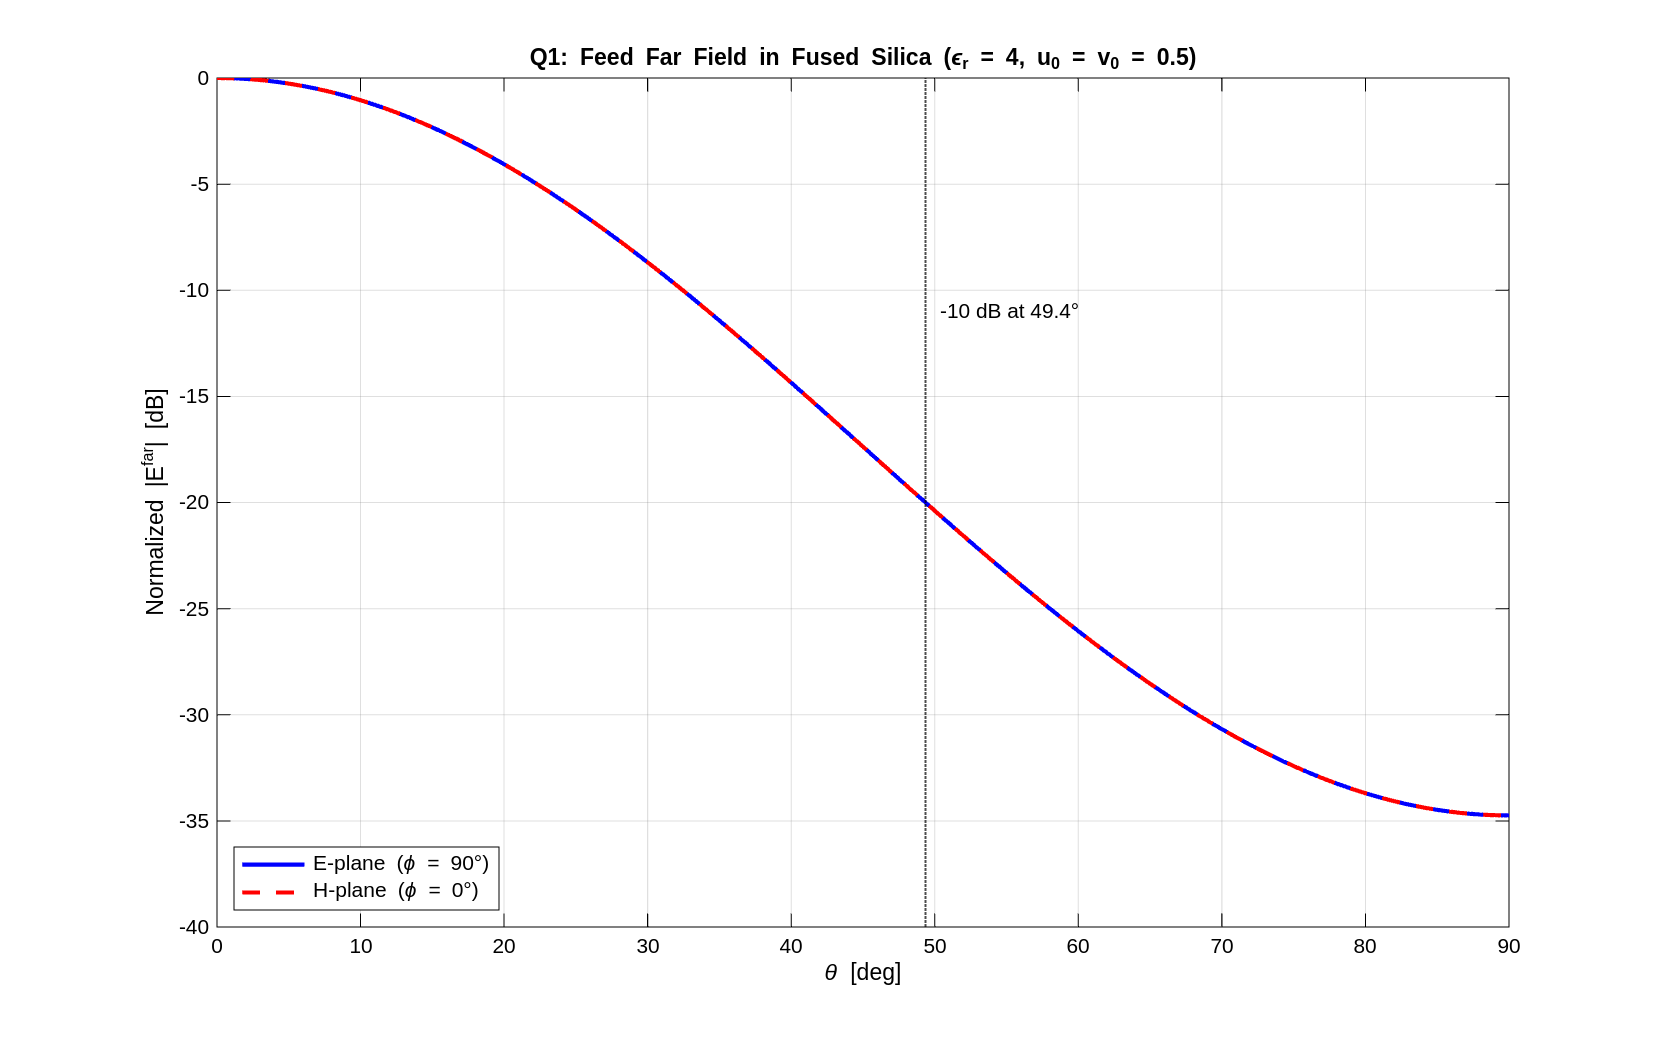
\includegraphics[width=0.85\textwidth]{figures/Q1_feed_farfield.png}
\caption{Normalized far-field pattern of the Gaussian feed in infinite fused silica ($\varepsilon_r = 4$, $u_0 = v_0 = 0.5$, \SI{200}{GHz}). E-plane and H-plane curves overlap due to the circular symmetry $u_0 = v_0$.}
\label{fig:q1}
\end{figure}

Observations from Figure~\ref{fig:q1}:
\begin{itemize}
\item The pattern is a smooth Gaussian roll-off with no sidelobes. The E-plane and H-plane curves are identical, confirming the circular symmetry of the feed for $u_0 = v_0$.
\item The polarization $(\sin\phi\,\hat{\theta} + \cos\phi\,\hat{\phi})$ is a Huygens-type source: in the E-plane it is purely $\hat{\theta}$-polarized, in the H-plane purely $\hat{\phi}$-polarized. This ensures the co-pol pattern is the same in both planes.
\item This circular symmetry will be broken when the lens is introduced (Q4, Q5), because the Fresnel transmission coefficients differ for TE and TM polarizations.
\end{itemize}

%% ====================================================================
\section{Q2: Fresnel Transmission Coefficients --- Flat Interface}
%% ====================================================================

The Fresnel transmission coefficients for a flat fused silica-to-air interface are:
\begin{equation}\label{eq:fresnel_tau}
\tau^\perp = \frac{2\zeta_0\cos\theta_i}{\zeta_0\cos\theta_i + \zeta_d\cos\theta_t}, \qquad \tau^\parallel = \frac{2\zeta_0\cos\theta_i}{\zeta_0\cos\theta_t + \zeta_d\cos\theta_i}
\end{equation}
where $\zeta_d = \zeta_0/\sqrt{\varepsilon_r}$ and Snell's law gives $\sqrt{\varepsilon_r}\sin\theta_i = \sin\theta_t$. The power transmission ratio is:
\begin{equation}\label{eq:power_trans}
\frac{P_t}{P_i} = |\tau|^2 \frac{\zeta_d\cos\theta_t}{\zeta_0\cos\theta_i} = 1 - |\Gamma|^2
\end{equation}

\begin{figure}[H]
\centering
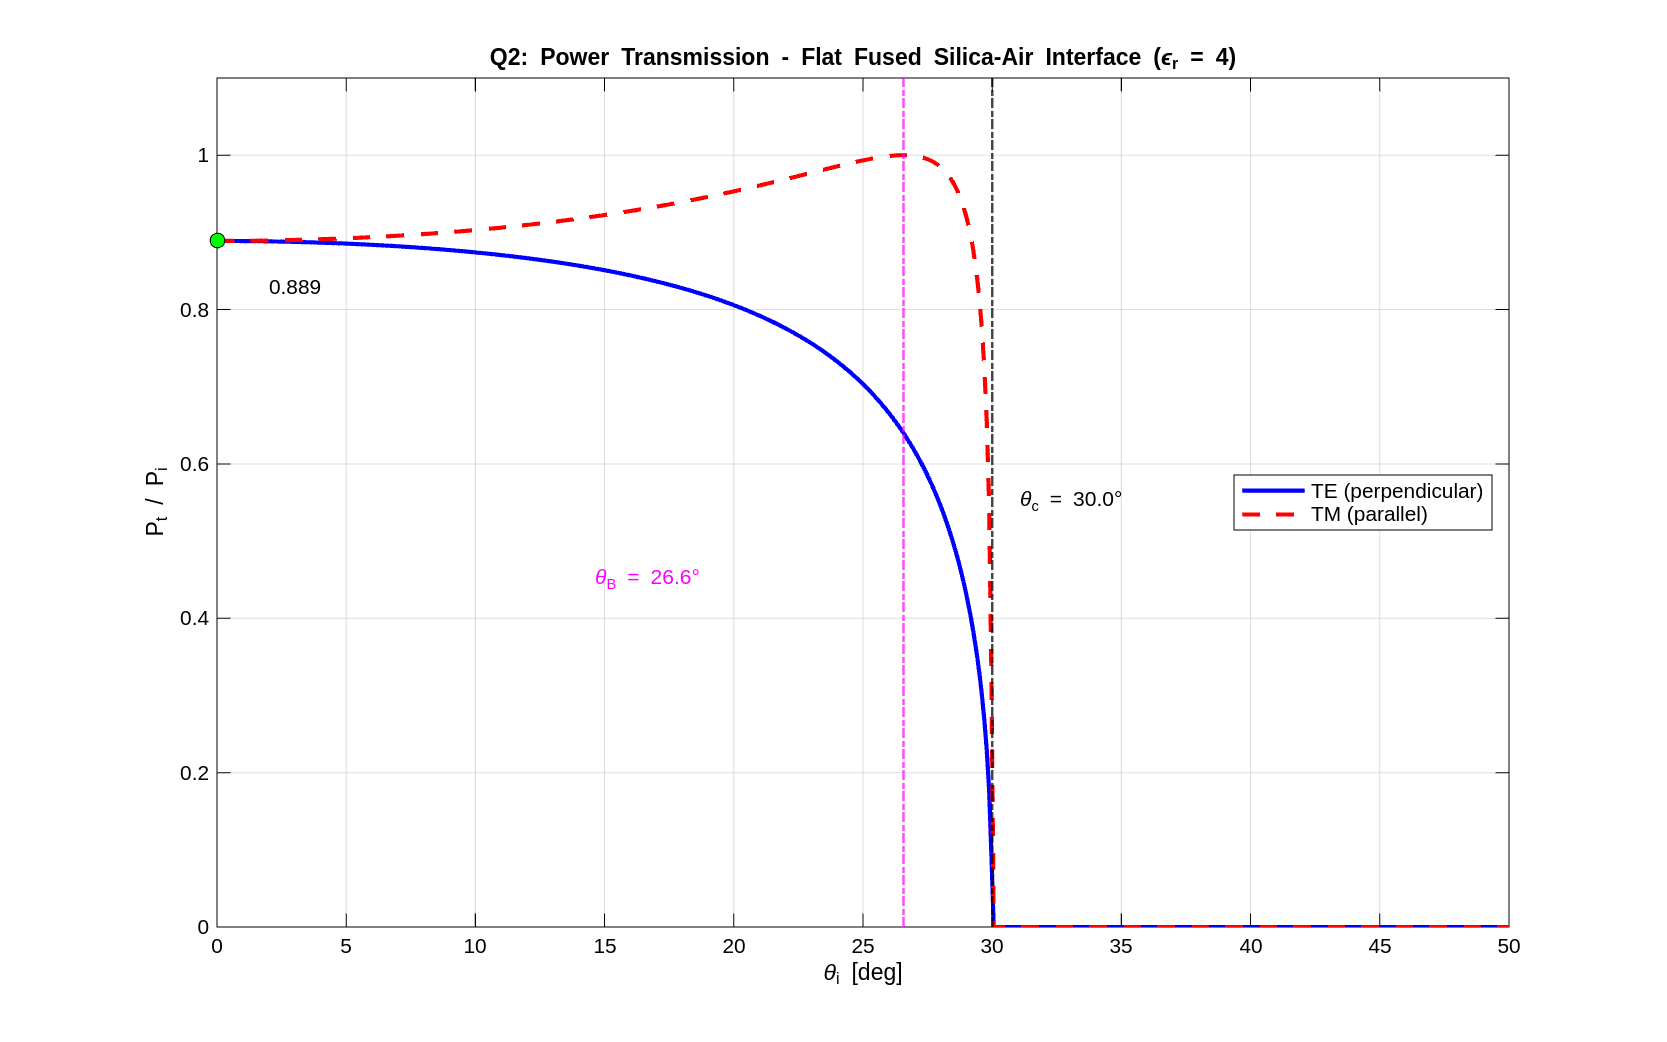
\includegraphics[width=0.85\textwidth]{figures/Q2_fresnel_flat.png}
\caption{Power transmission ratio $P_t/P_i$ vs.\ incidence angle for a flat fused silica--air interface ($\varepsilon_r = 4$), for TE and TM polarizations.}
\label{fig:q2}
\end{figure}

Observations from Figure~\ref{fig:q2}:
\begin{enumerate}
\item \textbf{Normal incidence} ($\theta_i = 0^\circ$): $P_t/P_i = 4n/(1+n)^2 = 8/9 \approx 0.889$ for both TE and TM ($n = \sqrt{\varepsilon_r} = 2$). About 11.1\% of power is reflected.

\item \textbf{Brewster angle} (TM only): $\theta_B = \arctan(1/\sqrt{\varepsilon_r}) = 26.6^\circ$. At this angle $\Gamma^\parallel = 0$ and TM transmission is complete ($P_t/P_i = 1$). No corresponding angle exists for TE, since $\Gamma^\perp$ increases monotonically with $\theta_i$.

\item \textbf{Critical angle}: $\theta_c = \arcsin(1/\sqrt{\varepsilon_r}) = 30.0^\circ$. Beyond this angle, total internal reflection occurs for both polarizations: $\sin\theta_t > 1$, $\theta_t$ becomes complex, and all power is reflected.

\item \textbf{Between Brewster and critical} (TM): $P_t/P_i$ drops from 1.0 back to 0 over a narrow $3.4^\circ$ range, demonstrating the rapid transition to total internal reflection.
\end{enumerate}

%% ====================================================================
\section{Q3: Fresnel Transmission Coefficients --- Elliptical Lens ($D = 9\lambda_0$)}
%% ====================================================================

On the elliptical lens surface, the local incidence angle depends on the elevation angle $\theta$ from the lower focus via:
\begin{equation}\label{eq:theta_i_lens}
\cos\theta_i = \frac{1 - e\cos\theta}{\sqrt{1 + e^2 - 2e\cos\theta}}
\end{equation}

The computed lens parameters for $D = 9\lambda_0 = \SI{13.5}{mm}$ are: $e = 0.500$, $a = \SI{7.794}{mm}$, $b = \SI{6.750}{mm}$, lens height $h = a(1+e) = \SI{11.691}{mm}$, and maximum lens angle $\theta_{\max} = \arctan(b/(ea)) = 60.0^\circ$.

\begin{figure}[H]
\centering
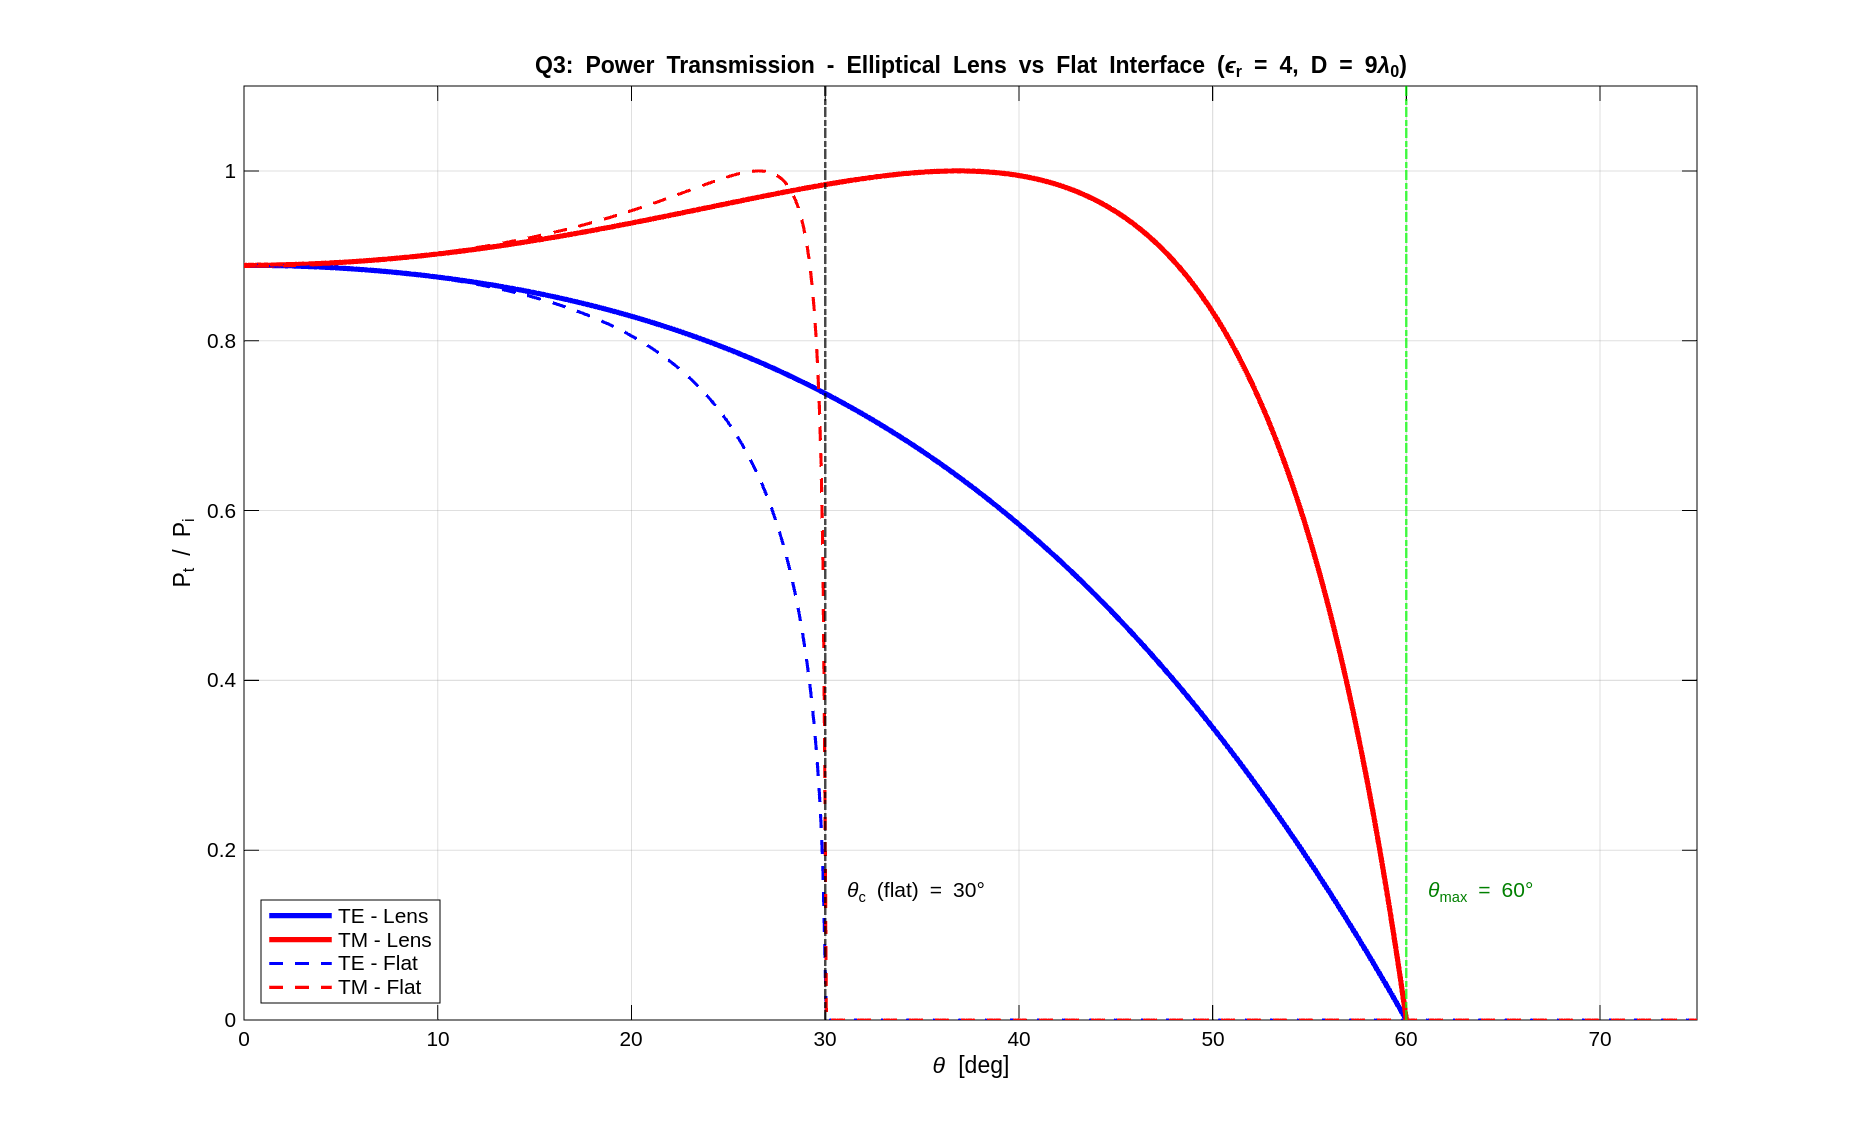
\includegraphics[width=0.85\textwidth]{figures/Q3_fresnel_lens.png}
\caption{Power transmission ratio vs.\ elevation angle $\theta$ for the elliptical lens (solid) compared with the flat interface (dashed). The lens extends significant transmission well beyond the flat-interface critical angle of $30^\circ$.}
\label{fig:q3}
\end{figure}

Observations from Figure~\ref{fig:q3}:
\begin{itemize}
\item At the top of the lens ($\theta = 0$), $\theta_i = 0^\circ$ and the transmission equals the flat normal-incidence value of 0.889 for both polarizations.
\item The elliptical curvature causes the local incidence angle to grow much more slowly than $\theta$ itself. At $\theta = 40^\circ$ (the truncation angle used in Q4--Q6), the local $\theta_i \approx 17^\circ$, still well below the critical angle.
\item The flat interface (dashed) shows total internal reflection at $\theta_i = 30^\circ$, but the lens maintains significant transmission well beyond $\theta = 30^\circ$. TM transmission (solid red) stays above 0.9 up to $\theta \approx 50^\circ$ due to the Brewster effect on the curved surface.
\item At $\theta_{\max} = 60^\circ$, the local incidence angle reaches exactly $30^\circ$ (the critical angle), and both polarizations drop to zero. This is a fundamental property of the elliptical lens with $e = 1/\sqrt{\varepsilon_r}$: the maximum lens angle always maps to the critical angle.
\item The key advantage of the elliptical geometry is clear: it extends the range of high transmission to much larger elevation angles compared to a flat interface, enabling wider feeds while maintaining good power transfer.
\end{itemize}

%% ====================================================================
\section{Q4: Aperture Current Distribution}
%% ====================================================================

The lens is truncated at $\theta_0 = 40^\circ$ with $\varepsilon_r = 4$, $D = 9\lambda_0$, and $u_0 = v_0 = 0.5$. The equivalent aperture currents are computed using the GO/PO method. The elliptical lens provides a spreading factor $S = 1$ (exact) and uniform phase $k_d r + k_0 r' = k_d a(1+e)$ across the aperture.

Since the equivalent electric and magnetic surface currents are orthogonal with the same distribution, the far field can be computed using only $\vec{J}_s$ with twice the amplitude:
\begin{align}
J_{s,x} &= -\frac{2}{\zeta_0}\frac{1}{r}\left[\tau^\parallel E_i^\theta\cos\phi - \tau^\perp E_i^\phi\sin\phi\right] \label{eq:Jsx}\\
J_{s,y} &= -\frac{2}{\zeta_0}\frac{1}{r}\left[\tau^\parallel E_i^\theta\sin\phi + \tau^\perp E_i^\phi\cos\phi\right] \label{eq:Jsy}
\end{align}

For the Huygens feed, $E_i^\theta = \sin\phi\cdot G(\theta)$ and $E_i^\phi = \cos\phi\cdot G(\theta)$, where $G(\theta)$ is the Gaussian envelope. In the principal planes this simplifies to:
\begin{itemize}
\item E-plane ($\phi = 90^\circ$): $J_y \propto \tau^\parallel \cdot G(\theta)/r$, \;$J_x = 0$
\item H-plane ($\phi = 0^\circ$): $J_y \propto \tau^\perp \cdot G(\theta)/r$, \;$J_x = 0$
\end{itemize}

\begin{figure}[H]
\centering
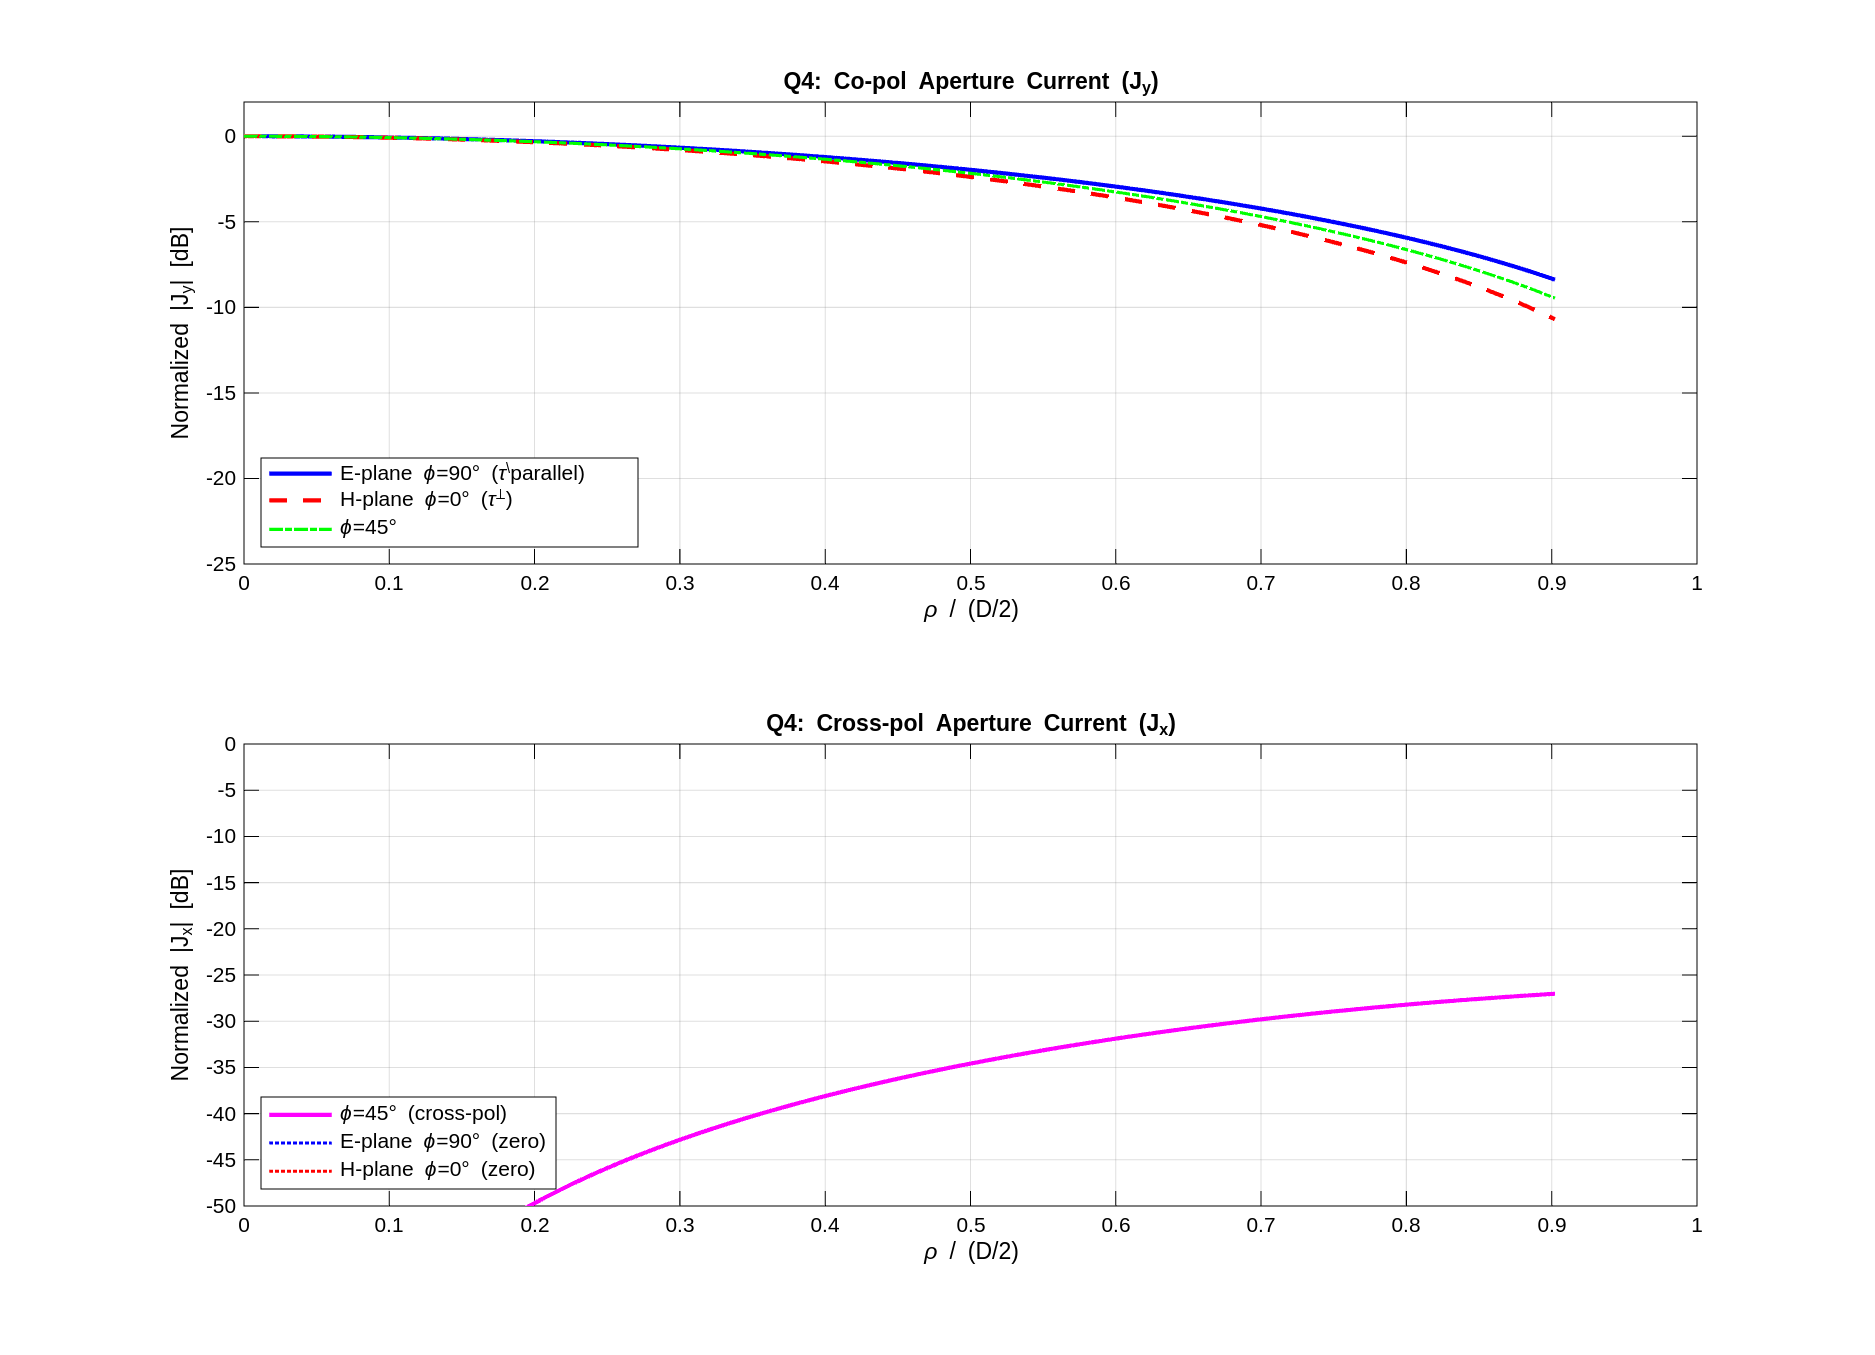
\includegraphics[width=0.85\textwidth]{figures/Q4_aperture_currents.png}
\caption{Normalized aperture current distribution. Top: co-pol component $J_y$ in the E-plane ($\tau^\parallel$), H-plane ($\tau^\perp$), and $\phi = 45^\circ$ cut. Bottom: cross-pol component $J_x$ at $\phi = 45^\circ$; $J_x$ is identically zero in the principal planes.}
\label{fig:q4}
\end{figure}

Observations from Figure~\ref{fig:q4}:
\begin{itemize}
\item \textbf{Co-pol} ($J_y$): The E-plane (governed by $\tau^\parallel$, TM) shows an edge taper of $-8.4$\,dB, while the H-plane (governed by $\tau^\perp$, TE) shows a steeper taper of $-10.7$\,dB. The TM coefficient benefits from the Brewster effect, maintaining higher transmission at oblique angles, hence the gentler taper in the E-plane.

\item \textbf{Cross-pol} ($J_x$): In the principal planes ($\phi = 0^\circ$ and $90^\circ$), the cross-pol is identically zero because the Huygens polarization aligns perfectly with the TE/TM decomposition axes. At $\phi = 45^\circ$, cross-pol appears at $-27.0$\,dB below co-pol, arising from the mismatch $\tau^\parallel \neq \tau^\perp$.

\item \textbf{Effect of feed pattern} (Q1): The Gaussian taper dominates the amplitude variation. At $\theta_0 = 40^\circ$, the feed itself is at about $-5$\,dB, which combined with the Fresnel coefficient variation and $1/r$ geometric taper produces the total 8--11\,dB edge taper.

\item \textbf{Effect of transmission coefficients}: Without Fresnel effects ($\tau^\perp = \tau^\parallel$), the aperture distribution would be perfectly circularly symmetric. The E/H asymmetry and the cross-pol generation are entirely due to $\tau^\perp \neq \tau^\parallel$.
\end{itemize}

%% ====================================================================
\section{Q5: Lens Far Field}
%% ====================================================================

The lens far field is computed via the free-space spectral Green's function applied to the aperture currents from Q4:
\begin{equation}\label{eq:lens_farfield}
\vec{E}^{far}_{lens}(\vec{r}) = jk_{zs}\,\tilde{\bar{G}}^{ej}_{fs}(k_{xs},k_{ys})\,\tilde{\vec{J}}_s(k_{xs},k_{ys})\,\frac{e^{-jk_0 r}}{2\pi r}
\end{equation}
where $\tilde{\vec{J}}_s$ is the 2D Fourier transform of the aperture currents, evaluated at the stationary phase point $(k_{xs},k_{ys}) = k_0(\sin\theta\cos\phi,\,\sin\theta\sin\phi)$. The computation uses a $301\times301$ aperture grid with 1001 far-field angle samples.

\begin{figure}[H]
\centering
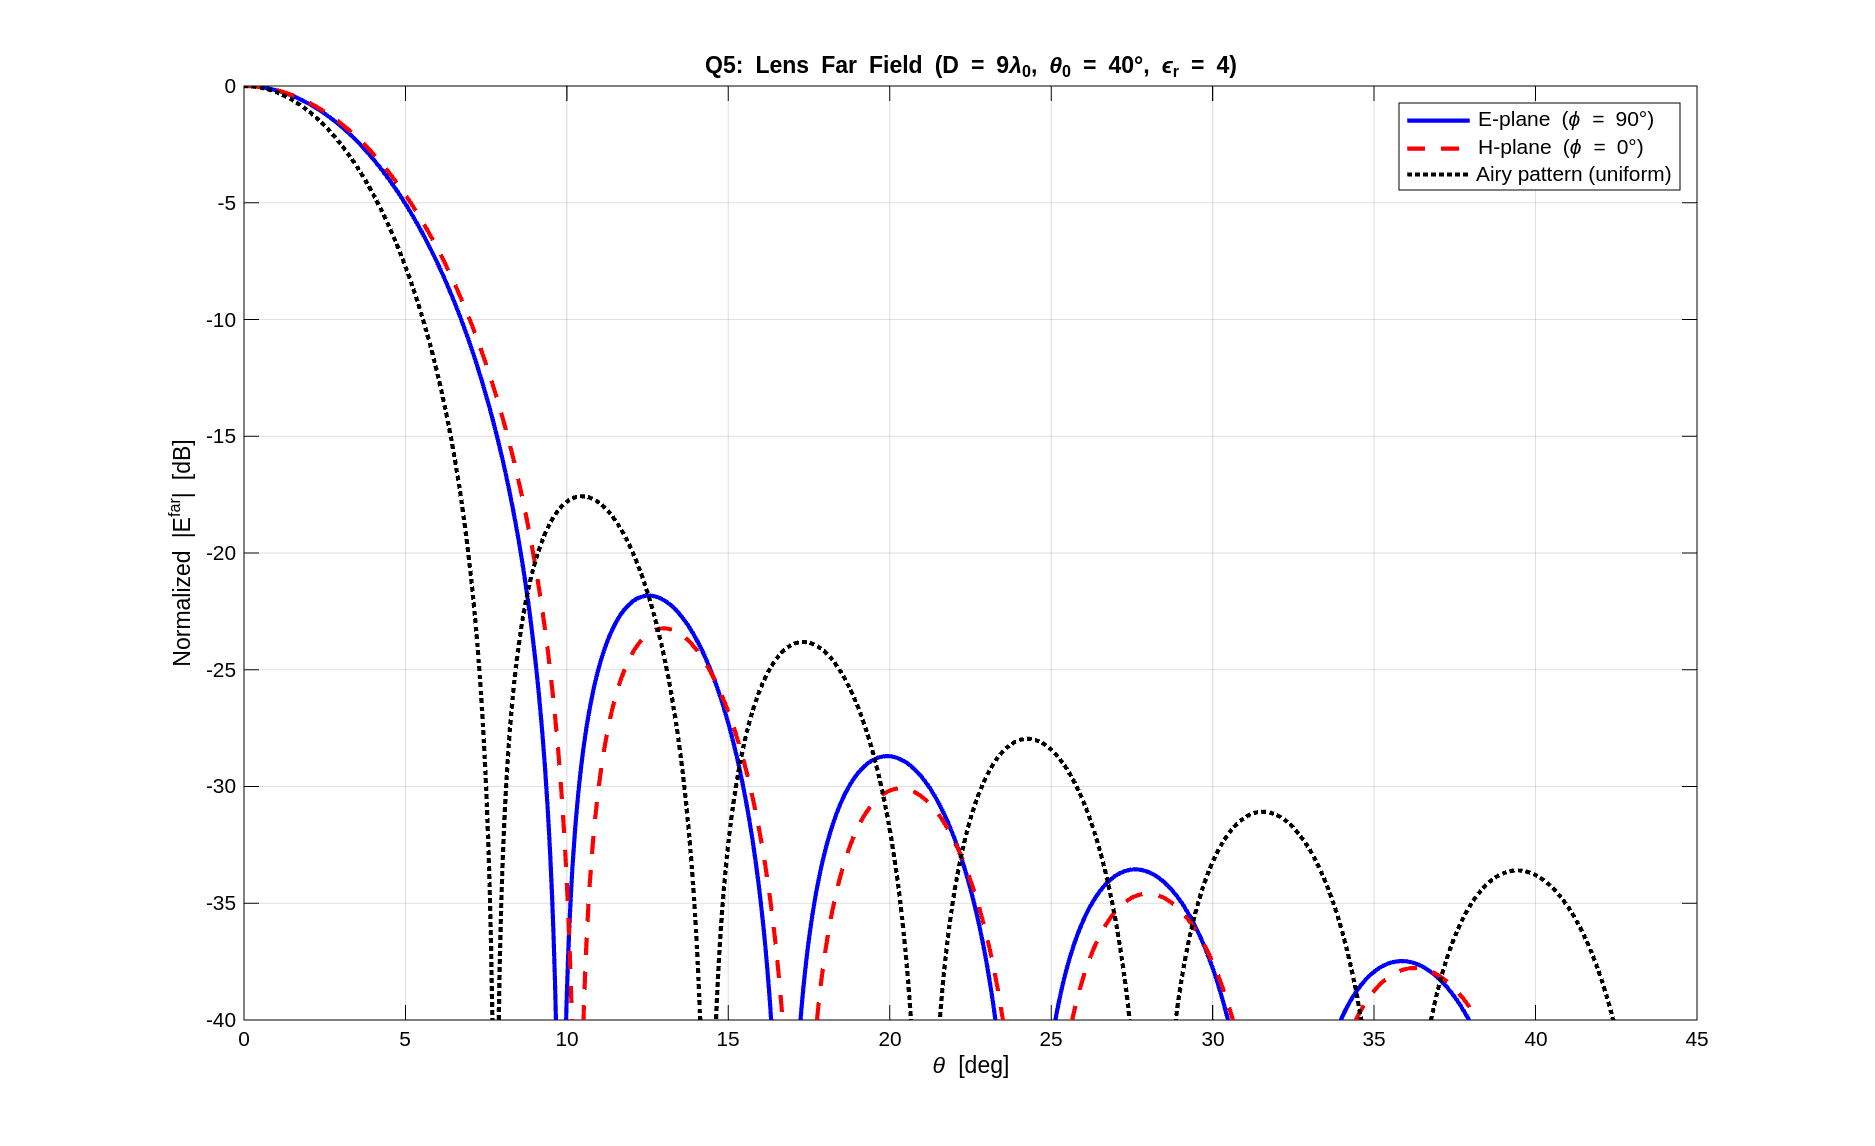
\includegraphics[width=0.85\textwidth]{figures/Q5_lens_farfield.png}
\caption{Normalized lens far-field pattern in the E-plane and H-plane, compared with the Airy pattern of a uniformly illuminated circular aperture of diameter $D = 9\lambda_0$.}
\label{fig:q5}
\end{figure}

Observations from Figure~\ref{fig:q5}:
\begin{enumerate}
\item \textbf{Wider main beam}: The first null of the lens pattern is at ${\sim}9^\circ$--$10^\circ$, compared to ${\sim}8^\circ$ for the Airy pattern. The Gaussian + Fresnel amplitude taper reduces the effective aperture size, broadening the main beam.

\item \textbf{Lower sidelobes}: The first sidelobe is approximately $-22$\,dB (E-plane) and $-26$\,dB (H-plane), well below the Airy first sidelobe at $-17.6$\,dB. The smooth taper acts as a window function that suppresses sidelobes at the cost of a wider main beam.

\item \textbf{E/H plane asymmetry}: The H-plane shows deeper nulls and lower sidelobes than the E-plane. This asymmetry is governed by:
\begin{itemize}
\item \textit{Primary cause}: $\tau^\perp \neq \tau^\parallel$. The E-plane co-pol uses $\tau^\parallel$ (TM, gentler taper $\to$ narrower beam, higher sidelobes), while the H-plane uses $\tau^\perp$ (TE, steeper taper $\to$ wider beam, lower sidelobes). This is consistent with the aperture current asymmetry observed in Q4 (Figure~\ref{fig:q4}).
\item \textit{Secondary cause}: The free-space SGF introduces a $\cos\theta$ factor difference between $E_\theta$ and $E_\phi$ projections.
\end{itemize}
\end{enumerate}

%% ====================================================================
\section{Q6: Directivity and Gain}
%% ====================================================================

The directivity is computed from the far-field radiation intensity integrated over the upper hemisphere on a $301\times181$ angular grid:
\begin{equation}\label{eq:directivity}
D = \frac{4\pi\,U_{\max}}{P_{rad}}, \qquad U(\theta,\phi) = |E_\theta|^2 + |E_\phi|^2
\end{equation}

The gain accounts for power lost to spillover and Fresnel reflection:
\begin{equation}\label{eq:gain}
G = D \cdot \eta_r, \qquad \eta_r = \frac{P^{lens}_{rad}}{P^{feed}_{rad}}
\end{equation}
where $\eta_r$ includes both spillover losses (feed power missing the lens) and Fresnel reflection losses at the lens surface.

\begin{table}[H]
\centering
\caption{Directivity, gain, and efficiency breakdown for the lens antenna of Q4.}
\label{tab:q6}
\begin{tabular}{@{}ll@{}}
\toprule
Parameter & Value \\
\midrule
$D_{\max}$ (uniform aperture, $(\pi D/\lambda_0)^2$) & \SI{29.0}{dBi} \\
Directivity $D$ & \SI{27.8}{dBi} \\
Gain $G = D \cdot \eta_r$ & \SI{27.0}{dBi} \\
\midrule
Spillover efficiency $\eta_s$ & 94.8\% \\
Reflection efficiency $\eta_{\text{refl}}$ & 87.8\% \\
Total $\eta_r = \eta_s \cdot \eta_{\text{refl}}$ & 83.3\% \\
Aperture efficiency $D/D_{\max}$ & 74.9\% \\
\bottomrule
\end{tabular}
\end{table}

The results in Table~\ref{tab:q6} can be interpreted as follows:
\begin{itemize}
\item The directivity is \SI{1.2}{dB} below $D_{\max}$, due to the amplitude taper from the Gaussian feed pattern and the Fresnel coefficient variation across the aperture.

\item The gain is a further \SI{0.8}{dB} below the directivity, due to the combined spillover and reflection losses.

\item The high spillover efficiency (94.8\%) is expected: the feed $-10$\,dB angle ($49.4^\circ$) is well beyond the lens truncation angle ($40^\circ$), so most feed power is intercepted by the lens.

\item The reflection efficiency (87.8\%) represents the average Fresnel loss across the lens surface, which is moderate for fused silica ($\varepsilon_r = 4$).

\item The overall aperture efficiency of 74.9\% is a good result for an unmatched dielectric lens antenna, and could be improved further with a quarter-wave matching layer ($\varepsilon_{r,m} = \sqrt{\varepsilon_r} = 2$, thickness $\lambda_m/4$), which would eliminate the broadside reflection and improve $\eta_{\text{refl}}$.
\end{itemize}

\end{document}
